\index{Linear time-invariant systems}{Linear time-invariant systems}
(LTI) are an important class of systems that can be analyzed easily in frequency domain. An LTI system is equivalent to \emph{\index{convolution}{convolution}} of the \emph{impulse response} of the system. The focus of this chapter is to learn more about what these concepts are. 

\section{Example: Running average filter}
Here's an example of a discrete-time system that you might use to smooth a noisy signal:
\begin{equation}
  y[n] = \frac{1}{15}\sum_{k=-7}^{7} x[n-k]\,\,.
  \label{eq:running_mean}
\end{equation}
What does this system do? It averages together 15 neighboring values of input signal $x[n]$. Figure \ref{fig:avg_filter} shows a demonstration of this system in action. The blue line indicates a noisy input signal $x[n]$, and the orange line depicts the output $y[n]$ of the running mean filter given in Equation \ref{eq:running_mean}. As you might expect, the output of the system is a smoother version of the input signal.
\begin{figure}
  \begin{center}
    \includegraphics[width=\textwidth]{ch10/figures/smoothing.png}
  \end{center}
  \caption{A running average filter is often used to smooth a noisy
    signal. You can find the Python code used to produce this example
    in \texttt{016\_smoothing/smoothing.py}.}
  \label{fig:avg_filter}
\end{figure}

\section{Finite impulse response filter}
\begin{marginfigure}

\begin{center}
  \begin{tikzpicture}[node distance=3cm,auto,>=latex']
    \node [int] (a) {LTI};
    \node (b) [left of=a, coordinate] {a};
%    \node (c) [below=a,node distance=3cm] {a};

%\node [int, pin={[init]above:$p_0$}] (c) [right of=a] {$\frac{1}{s}$};
    \node [coordinate] (end) [right of=a]{};
    \path[->] (b) edge node {$x[n]$} (a);
    \path[->] (b) edge node [below]{$\delta[n]$} (a);

%\path[->] (a) edge node {$v$} (c);
    \draw[->] (a) edge node {$y[n]$} (end) ;
    \draw[->] (a) edge node [below]{$h[n]$} (end) ;

\end{tikzpicture}
\end{center}
\caption{Discrete-time LTI systems are characterized by an impulse response $h[n]$, which is the response of the LTI system to a unit impulse signal.}
\end{marginfigure}

The previous system shown in Equation \ref{eq:running_mean} is a special case of a more general type of a discrete-time LTI system, known as a Finite Impulse Response (FIR) filter. This type of signal is often used in digital signal processing. An FIR filter is defined as follows:
\begin{equation}
  \boxed{
    y[n] = \sum_{k=-M}^{N} b_k x[n-k]\,\,.
  }
  \label{eq:fir_filter}
\end{equation}
The coefficients $b_k \in \mathbb{C}$ here are constant valued coefficients. As the name implies, there is a finite number of non-zero coefficients $b_k$. In the case of the running average filter in Equation \ref{eq:running_mean}, there would be 15 coefficients, which are all $b_k=1/15$.

\section{General discrete-time LTI system}
What if we allow there to be infinitely many coefficients for the system given in Equation \ref{eq:fir_filter}? We get the following:
\begin{equation}
    y[n] = \sum_{k=-\infty}^{\infty} b_k x[n-k] = \sum_{k=-\infty}^{\infty} b[k] x[n-k]\,\,.
\end{equation}
This turns out to be the general representation for arbitrary discrete-time LTI systems! In this case, it makes sense to think of the infinitely many coefficients $b_k$ as a signal $b[k]$.

For discrete-time LTI systems in general, the output of a system is given by a discrete-time convolution sum of the input signal $x[n]$ with an impulse response $h[n]$:

\begin{marginfigure}
  \begin{center}
          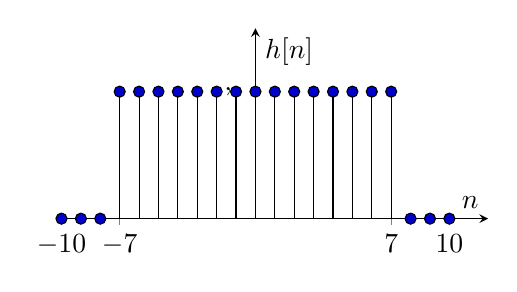
\begin{tikzpicture}
          \begin{axis}[width=7cm,height=4cm,ymin=0,xmin=-10,ymax=0.1,xmax=12,
         xtick={-10,-7,0,7,10},
              ytick={0,1,2,3},
              ytick={0,0.0667},
              yticklabel={,,},
          ylabel={$h[n]$},
      xlabel={$n$}, axis lines = center]
     \addplot+[ycomb,color=black] plot coordinates {(-10,0)(-9,0)(-8,0)(-7,0.0667)(-6,0.0667)(-5,0.0667)(-4,0.0667)(-3,0.0667)(-2,0.0667)(-1,0.0667)(0,0.0667)(1,0.0667)(2,0.0667)(3,0.0667)(4,0.0667)(5,0.0667)(6,0.0667)(7,0.0667)(8,0)(9,0)(10,0)};
  \end{axis}
  \end{tikzpicture}
  \end{center}
  \caption{The impulse response of the 15 point running mean filter described in Equation \ref{eq:running_mean}.}
\end{marginfigure}

\begin{equation}
  \boxed{
    y[n] = \mathcal{T}\{x[n]\}=\sum_{k=-\infty}^{\infty} h[k] x[n-k]\,\,.
  }
  \label{eq:conv_dlti}
\end{equation}
The impulse response is defined as follows:
\begin{equation}
  \boxed{
    h[n] = \mathcal{T}\{\delta[n]\}\,\,.
  \label{eq:conv_ireq}    
    }
\end{equation}
It is hopefully easy to see that Equation \ref{eq:conv_dlti} is valid for all LTI systems. %This was already briefly discussed earlier in the chapter on Fourier transforms.

A linear system $\mathcal{T}\{\cdot\}$\footnote{If linearity applies for two input signals $\mathcal{T}\{\alpha_1 s_1[n] + \alpha_2 s_2[n]\} = \alpha_1 \mathcal{T}\{s_1[n]\}+\alpha_2 \mathcal{T}\{s_2[n]\}$, it also applies for linear combinations of three or more signals.} must by definition satisfy the following relation:
\begin{equation}
  \mathcal{T}\left\{\sum_{k=-\infty}^{\infty} \alpha_k s_k[n]\right\} = \sum_{k=-\infty}^{\infty} \alpha_k \mathcal{T}\{s_k[n]\}\,\,.
  \label{eq:linearity_gen}
\end{equation}
Here $\alpha_k \in \mathbb{C}$ are arbitrary constants and $s_k[n]$ are arbitrary signals.

Time-invariance of system $\mathcal{T}\{\cdot\}$ on the other hand implies that for any time shift $k$ in input, the output is correspondingly time shifted. This is valid for any input signal $x[n]$:
\begin{equation}
y[n-k] = \mathcal{T}\{x[n-k]\}\,\,,
\end{equation}
if 
\begin{equation}
y[n]=\mathcal{T}\{x[n]\}\,\,.
\end{equation}
It is possible to represent any signal $x[n]$ with the help of time-shifted unit impulse signals\sidenote{Recall that the discrete-time unit impulse is defined as: 
\begin{equation}
\delta[n] = \left\{
  \begin{array}{rcr}
    1 & \mathrm{when} & n=0 \\
    0 & \mathrm{otherwise} & \\
  \end{array}
\right.\,\,.
\end{equation}

It is the discrete-time equivalent of a Dirac delta function. The unit impulse is shown in Figure \ref{fig:dt_unit_impulse}.
}:
\begin{equation}
  x[n] = \sum_{k=-\infty}^{\infty} x[k]\delta[n-k]\,\,.
\end{equation}
Linearity implies that:
\begin{equation}
\mathcal{T}\{x[n]\} = \mathcal{T}\left\{\sum_{k=-\infty}^{\infty}x[k]\delta[n-k]\right\} = \sum_{k=-\infty}^{\infty}x[k] \mathcal{T}\{\delta[n-k]\}\,\,.
\end{equation}
\if 0
\begin{marginfigure}
\begin{center}
    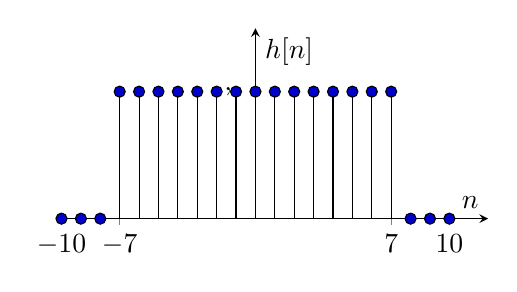
\begin{tikzpicture}
      \begin{axis}[width=7cm,height=4cm,ymin=0,xmin=-10,ymax=0.1,xmax=12,
                   xtick={-10,-7,0,7,10},
                  ytick={0,1,2,3},
             ytick={0,0.0667},
             yticklabel={,,},
             ylabel={$h[n]$},
             xlabel={$n$}, axis lines = center]
        \addplot+[ycomb,color=black] plot coordinates {(-10,0)(-9,0)(-8,0)(-7,0.0667)(-6,0.0667)(-5,0.0667)(-4,0.0667)(-3,0.0667)(-2,0.0667)(-1,0.0667)(0,0.0667)(1,0.0667)(2,0.0667)(3,0.0667)(4,0.0667)(5,0.0667)(6,0.0667)(7,0.0667)(8,0)(9,0)(10,0)};
      \end{axis}
     \end{tikzpicture}
\end{center}
\caption{The impulse response of the 15 point running mean filter described in Equation \ref{eq:running_mean}.}
\end{marginfigure}
\fi
\noindent The equation above is the same as Equation \ref{eq:linearity_gen} with $s_k[n] = \delta[n-k]$ and $\alpha_k=x[k]$.  Due to time-invariance,
we can relate the impulse response $h[n]$ delayed by $k$ to the term
on the right-hand side above. If a unit impulse fed into the system is
\begin{equation}
h[n] = \mathcal{T}\{\delta[n]\},
\end{equation}
\begin{marginfigure}
  \begin{center}
    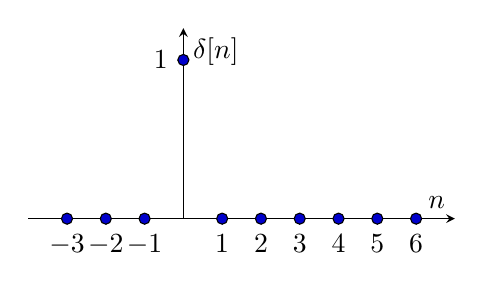
\begin{tikzpicture}
      \begin{axis}[width=7cm,height=4cm,ymin=0,xmin=-4,ymax=1.2,xmax=7,
                   xtick={-3,-2,-1,0,1,2,3,4,5,6},
                   ytick={0,1,2,3},
                   ylabel={$\delta[n]$},
                   xlabel={$n$}, axis lines = center]
          \addplot+[ycomb,color=black] plot coordinates {(-3,0) (-2,0) (-1,0) (0,1) (1,0) (2,0) (3,0) (4,0) (5,0) (6,0)};
      \end{axis}
     \end{tikzpicture}
     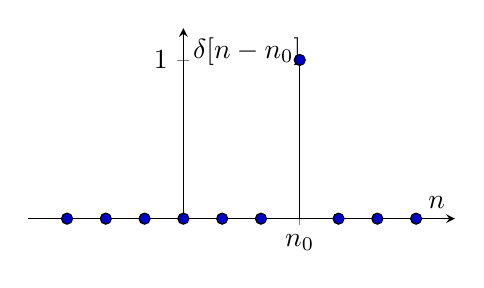
\begin{tikzpicture}
        \begin{axis}[width=7cm,height=4cm,ymin=0,xmin=-4,ymax=1.2,xmax=7,
          xtick={3},
          xticklabels={$n_0$},
          ytick={0,1,2,3},
          ylabel={$\delta[n-n_0]$},
          xlabel={$n$}, axis lines = center]
          \addplot+[ycomb,color=black] plot coordinates {(-3,0) (-2,0) (-1,0) (0,0) (1,0) (2,0) (3,1) (4,0) (5,0) (6,0)};
        \end{axis}
      \end{tikzpicture}
  \end{center}
  \caption{Discrete-time unit impulse signal $\delta[n]$ and a time-shifted version $\delta[n-n_0]$ centered at $n=n_0$.}
  \label{fig:dt_unit_impulse}
\end{marginfigure}
then a time-shifted unit impulse corresponds to a time-shifted output:
\begin{equation}
h[n-k] = \mathcal{T}\{\delta[n-k]\}\,\,.
\end{equation}
Therefore, the output of an LTI system for an arbitrary input signal
$x[n]$ can be expressed using the impulse response $h[n]$ as follows:
\begin{equation}
  y[n] = \sum_{k=-\infty}^{\infty} x[k]h[n-k].
  \label{eq:convolution_intro}
\end{equation}
This type of an equation is known as a discrete-time convolution sum. We have now shown that any discrete-time LTI system can be represented with such a convolution sum. Note that Equation \ref{eq:convolution_intro} isn't quite yet the same as Equation \ref{eq:conv_dlti}. We will later show in Equation \ref{eq:commutative_convolution_proof} that the convolution sum is commutative, i.e., that
\begin{equation}
 \sum_{k=-\infty}^{\infty} x[k]h[n-k] = \sum_{k=-\infty}^{\infty} h[k]x[n-k].
\end{equation}
Which completes the proof.

\subsection{Example: Impulse response of an FIR filter}
An FIR filter (Equation \ref{eq:fir_filter}) has the following impulse response:
\begin{equation}
h[n] = \sum_{k=-M}^{N} b_k \delta[n-k]\,\,.
\end{equation}
The signal $h[n]$ contains the values of the filter coefficients $h[n]=b_n$. Since there are a finite number of coefficients $b_k$, the impulse response $h[n]$ has non-zero values only in a finite range of samples. This is also where the name ``finite impulse response'' comes from.
\begin{marginfigure}
\begin{center}
  \begin{tikzpicture}[node distance=2cm,auto,>=latex']
    \node [int] (a) {FIR filter ($b_k$)};
    \node (b) [left of=a, coordinate] {a};
%    \node (c) [below=a,node distance=3cm] {a};

%\node [int, pin={[init]above:$p_0$}] (c) [right of=a] {$\frac{1}{s}$};
    \node [coordinate] (end) [right of=a]{};
    \path[->] (b) edge node {$\delta[n]$} (a);
    %\path[->] (a) edge node {$v$} (c);
    \draw[->] (a) edge node {$h[n]$} (end) ;
\end{tikzpicture}
\end{center}
\caption{The impulse response of an FIR filter is a signal that contains the coefficients. For a finite number of coefficients $b_k$, the length of the non-zero portion of the impulse response is finite and hence the name FIR.}
\end{marginfigure}


\section{Impulse response}
Linear time-invariant (LTI) systems are fully characterized by an \index{impulse response} impulse response $h(t)$. This impulse response is obtained by feeding a unit impulse into the LTI system:
\begin{equation}
\boxed{
h(t) = \mathcal{T}\{\delta(t)\}\,\,.
}
\end{equation}
Using an impulse response, it is possible to represent the output of any LTI system as a convolution between the impulse response and the input signal.
\begin{equation}
\boxed{
y(t) = \mathcal{T}\{x(t)\} = h(t)*x(t) = \int_{-\infty}^{\infty} h(\tau)x(t-\tau)d\tau\,\,.
}
\end{equation}
Let's prove this. We'll first need to represent an arbitrary signal as a sum of unit impulses:
\begin{equation}
x(t)  = \int_{-\infty}^{\infty} x(\tau) \delta(t-\tau) d\tau\,\,.
\end{equation}
One way to think of this integral is that the unit impulse $\delta(t-\tau)$ ``selects'' the value of $x(\tau)$ where $\tau=t$. Another way to think of this is that the Dirac delta functions form a set of basis functions for representing the signal $x(t)$.

\tikzstyle{int}=[draw, minimum size=2em]
\tikzstyle{init} = [pin edge={to-,thin,black}]

\begin{marginfigure}
\begin{center}

  \begin{tikzpicture}[node distance=3cm,auto,>=latex']

    \node [int] (a) [align=center]{LTI };
    \node (b) [left of=a, coordinate] {a};
%    \node (c) [below=a,node distance=3cm] {a};

%\node [int, pin={[init]above:$p_0$}] (c) [right of=a] {$\frac{1}{s}$};
    \node [coordinate] (end) [right of=a]{};
    \path[->] (b) edge node {$\delta(t)$} (a);
  %  \path[->] (b) edge node [below]{$\delta(t)$} (a);

%\path[->] (a) edge node {$v$} (c);
    \draw[->] (a) edge node {$h(t)$} (end) ;
 %   \draw[->] (a) edge node [below]{$h(t)$} (end) ;

\end{tikzpicture}

\end{center}
\caption{A linear time-invariant system is characterized by an impulse response.}
\end{marginfigure}

First of all, you may recall that linearity of system $\mathcal{T}\{\cdot\}$ implies that:
\begin{equation}
\mathcal{T}\{c_1 \delta(t-\tau_1) + c_2 \delta(t-\tau_2)\} = c_1 \mathcal{T}\{\delta(t-\tau_1)\}+ c_2 \mathcal{T}\{\delta(t-\tau_2)\}\,\,.
\end{equation}
Here I've used $\delta(t-\tau_1)$ and $\delta(t-\tau_2)$ as two different input signals. The terms $c_1,c_2\in \mathbb{C}$ are arbitrary complex valued constants.

Linearity must therefore also apply for the linear combination of an arbitrary number of inputs:
\begin{equation}
\mathcal{T}\left\{\sum_n x_n \delta(t-\tau_n)\right\} = \sum_n x_n \mathcal{T}\{\delta(t-\tau_n)\}\,\,.
\end{equation}
Linearity can be extended even further into a continuous linear combination:
\begin{equation}
\mathcal{T}\left\{\int_{-\infty}^{\infty} x(\tau)\delta(t-\tau)d\tau\right\} = \int_{-\infty}^{\infty} x(\tau) \mathcal{T}\{\delta(t-\tau)\} d\tau\,\,.
\end{equation}
We can simplify the right-hand side and get:
\begin{equation}
\int_{-\infty}^{\infty} x(\tau) \mathcal{T}\{\delta(t-\tau)\} d\tau = \mathcal{T}\left\{x(t)\right\}\,\,.
\end{equation}
In order to simplify the left-hand side, we have to rely on the property of \emph{time-invariance}. That is:
\begin{equation}
h(t) = \mathcal{T}\{\delta(t)\} \Rightarrow h(t-\tau) = \mathcal{T}\{\delta(t-\tau)\}\,\,.
\end{equation}
This now completes our proof:
\begin{equation}
y(t)=\int_{-\infty}^{\infty} x(\tau) h(t-\tau) d\tau = \mathcal{T}\left\{x(t)\right\}\qed\,\,.
\end{equation}
The output of a linear time-invariant system $y(t)=\mathcal{T}\{x(t)\}$ is a convolution of the system's impulse response $h(t)=\mathcal{T}\{\delta(t)\}$ with the input signal $x(t)$ fed into the system.

\section{Frequency response}
It is possible to view an LTI system as a filter, which modifies each frequency component of the input signal. How each frequency component of the input signal is modified, is determined by the Fourier transform of the impulse response of the LTI system, which we will call \index{frequency response} frequency response $\Hiw$.

Recall that every LTI system is characterized by an impulse response:
\begin{equation}
h(t) = \mathcal{T}\{\delta(t)\}\,\,.
\end{equation}
We also know that the output of the LTI system is a convolution between the input signal $x(t)$ and the impulse response, which is a multiplication in frequency domain:
\begin{equation}
y(t) = h(t)*x(t) \xleftrightarrow{\mathcal{F}} \hat{y}(\omega) = \Hiw \hat{x}(\omega)\,\,.
\end{equation}
The frequency response is therefore the Fourier transform of the impulse response of the LTI system:
\begin{equation}
\boxed{
\Hiw = \int_{-\infty}^{\infty} h(\tau)e^{-i\omega \tau}  d\tau\,\,.
}
\end{equation}
The absolute value $|\Hiw|$ is called the \index{magnitude response} magnitude response, and the phase angle $\angle \Hiw$ is called the \index{phase response} phase response. These determine how the LTI system modifies the amplitude and phase of each spectral component of the signal.
